\documentclass[12pt]{article}

\usepackage[utf8]{inputenc}
\usepackage[english]{babel}
\usepackage{fancyhdr}
\usepackage{graphicx}
\graphicspath{ {./images/} }
\usepackage{titling}
\usepackage{wrapfig}
\usepackage{float}
\usepackage[table,xcdraw]{xcolor}
\usepackage{blindtext}
\usepackage{setspace}
\usepackage{listings}
\usepackage{tocloft}
\usepackage{placeins}
\usepackage[titletoc]{appendix}
\usepackage{etoolbox}
\usepackage{setspace}
\usepackage{makecell, caption}
\renewcommand\theadfont{\normalsize\bfseries\boldmath}
\usepackage{siunitx}
\sisetup{detect-weight, range-phrase=/, range-units = single}
\usepackage{lipsum}
\usepackage{amsmath,amssymb}
\usepackage{caption}
\usepackage{subcaption}
\usepackage{commath}
\usepackage{float}
\usepackage{epigraph} 

\usepackage[T1]{fontenc}                
\usepackage{booktabs}

\usepackage[table,xcdraw]{xcolor}
\doublespacing
\usepackage[
    backend=biber,
    style=mla-new,
    citestyle=authoryear
    ]{biblatex}
\addbibresource{sources.bib}

\usepackage{geometry}
 \geometry{
 a4paper,
 left=20mm,
 right=20mm,
 bottom=25mm,
 top=25mm,
 }

\pagestyle{fancy}
\fancyhf{}
\chead{
    Russian Oil and Gas Exports:  EU Sanctions and the Aftermath of the Ukrainian Invasion 
    }
\rfoot{Page \thepage}
 
 \begin{document}
 

\thispagestyle{empty}

 \begin{center}
            \large{
                \textsc{
                    Russian Oil and Gas Exports:  EU Sanctions and the Aftermath of the Ukrainian Invasion
                    }
            }
      
      \vspace{2cm}
      
      \rule[6pt]{450pt}{0.5pt}
      
      \large{
        \textit{
            \textbf{Research Question:} 
            To what extent have European Union sanctions on crude oil and natural gas imports from Russia impacted the corresponding Russian export flows since the start of the Ukrainian invasion?
            }
        }
      
      \rule[6pt]{450pt}{0.5pt}
      
      \vspace{1cm}
      
      Economics Extended Essay
      
      \vspace{10cm}
      
      Personal code: kbj419 \\ \\
      Word count: 3998
 \end{center}
 
 
 \pagebreak
  
 \tableofcontents 
 
 \pagebreak
 
 \section{Introduction}

 
 Years of tension culminated on the 24th of February, 2022, when Russian forces conducted the invasion of Ukraine. The world watched in shock as Ukrainian citizens fled their homeland and civilians joined the resistance against the Russian army. The immediate response from world leaders in the European Union (EU) was sanctions - if the Russian economy crashed, they wouldn't be able to fund the war. However, in a global and interdependent economy, how much could this really have affected Russia? This essay explores \textbf{the extent to which European Union sanctions on crude oil and natural gas imports from Russia have impacted corresponding Russian exports since the start of the Ukrainian invasion.}
 
 In 2021, Russia's natural gas production accounted for 17.4\% of world supply and almost 40\% of the EU's supply, while their crude oil production was 13.4\% of world supply and 25\% of the EU's supply (\citeauthor{bp_2022}). Energy prices are a key driver of production costs in the economy. The European Union's imposition of sanctions as a protectionist measure on their primary oil and natural gas supplier and one of the largest producers in the world, namely Russia, created complex arrangements amid surging energy prices (\citeauthor{ember_2023}). This highlights the significance of the relationship between the EU and Russia due to their energy interdependence for both the EU's supply, and a key source of demand for Russia's crude oil and natural gas. As a result of Russia's attack on Ukraine, the EU took the long term decision to reduce its dependency on Russian energy, influencing the selection of trade partners and trade flows for both the EU and Russia. Due to the nature of these tightly interconnected transnational economic relations, EU sanctions not only impact the Russian economy, but also the European energy markets. Accordingly, it is important to understand how EU energy sanctions affect the export flows of Russian crude oil and natural gas. This essay analyses this issue taking an international macroeconomic approach and drawing upon multiple data sources to determine the impact of EU sanctions on Russian crude oil and natural gas exports.
 

\subsection{Literature Review}

As a result of the Russo-Ukrainian war, which began during February of 2014, the EU has had ongoing involvement in sanctions against Russia. An understanding of the history of sanctions in the energy sector and of the war to date will help clarify both the context of the current sanctions imposed in 2022 and the efficacy of previous sanctions.

The 2014 energy sanctions forbid EU cooperation and investment in Russia's extractive industry (\citeauthor{the_council_of_the_european_union_2014}). However, these sanctions exempted natural gas due to the EU's heavy dependency on Russian supply (\citeauthor{szczepański_2015}): Due to limited transportation options aside from existing pipelines, natural gas is not easy to substitute. In spite of the sanctions, Russian crude oil production has continued to increase, although falling oil prices have resulted in lower revenue from crude exports (\citeauthor{russell_2016}). Nonetheless, Russia is heavily dependent on Western technology: A high proportion of their off-shore hydrocarbon extraction technology is sourced from Western companies. This implies potentially serious long-term effects for production from these sanctions (\citeauthor{strategic_comments_2015}). Somewhat surprisingly, there has been a slight decrease in Russia's natural gas production and export volumes, which could be indirectly due to certain technological constraints related to the sanctions.

From the long-term effects of these 2014 sanctions, it is clear that Russian crude oil trade suffered little consequence from sanctions due to the nature of the transportability of crude oil, hinting at the likely similar long-term effects of sanctions imposed on crude oil in 2022, following this same pattern where Russia is able to substitute its trade partners, but possibly to a larger extent. However, it is important to note what Russia was unable to substitute in 2014 - namely, their natural gas export trade partners because of the limitations of natural gas transportation without sufficient technology which is what the 2014 sanctions targeted. 

 \subsection{Methodology}
 To determine how EU sanctions impacted Russian crude oil and natural gas exports, first we have to analyse the market for Russian crude oil and natural in the EU before the invasion. The proportion of Russia's exports of both of these products that were sold to Europe will be determined using statistics for volumes of crude oil and natural gas imported by the EU relative to Russia's total production. Using 2021 as a base year will allow us to analyse post-pandemic results. 

After determining Russia's crude oil and natural gas export flows to the EU prior to the invasion, this essay will analyse how the EU sanctions impacted this industry in Russia. To understand both the short term and long term outlook for the Russian crude oil and natural gas industry, the first step is to determine the sanctions imposed and their time frames. Then, the changes in EU imports of Russian crude oil and natural gas as of February 5th, 2023, with a focus on analysing the effect of the sanctions before the price cap on Russian oil products effective as of February 5th (\citeauthor{meredith_2023}), will be examined. Thirdly, the Russian crude oil and natural gas production volume and trade partners following the invasion will be investigated, seeing if the sanctions affected production while also examining Russian revenues from crude oil and natural gas to analyse how price changes and costs of production have impacted the Russian industries. The final look on Russian exports and trade partners for crude oil and natural gas will reveal how the Russian economy has adapted. 

An understanding of protectionist policies from the European allows an analysis of how the EU has been able to change their import sources. At the same time, the fundamental nature of the EU as a trade bloc will be analysed against the new trade partners Russia forms due to of these sanctions. Furthermore, analysing how the elasticity of goods varies with time allows for an understanding of how the global dependency on energy causes changes in prices in the short-term that are not necessarily maintained in the long-term. The concept of interdependency weaves through the economic theory in this essay, demonstrating the complex nature of the relationship between the EU and Russia. 

 An important limitation in this investigation is that only the effect of the sanctions are being analysed, which are not the unique driver of the state of the Russian economy. In addition, the Ukrainian invasion is taken simply as a context for the sanctions, and the effects of the invasion itself (including, but not limited to, military spending and civil unrest) are not being taken into account. Furthermore, this investigation is limited in the diversity of the sources accessed: While a large number of sources are used to obtain statistics to analyse the Russian oil and gas industry, they were all Western-based due to language barriers in finding and interpreting other sources. Before each source was used, this research always evaluated against other sources to corroborate reported values. Nonetheless, these values were reported by external companies, and by not Russia itself. Primary research was not included due to limitations in its accessibility, but is justified by the abundance of secondary data available. 


\section{Export Flows Before the Ukrainian Invasion}
The European Union and Russia have a highly interdependent relationship in relation to crude oil and natural gas with the EU heavily relying on Russia for supply, but also, with the EU having been a key customer for Russia. In 2021, the EU imported 24.8\% of their crude petroleum oil and 39.3\% of their natural gas from Russia, as shown in Figure \ref{fig:eu 21 flows} (\citeauthor{eurostat_2022}). Similarly, Russia has been historically dependent on the EU as a key customer for its crude oil and natural gas exports. In 2021, 49\% of crude oil exports and 74\% of natural gas exports were sold to the EU, as shown in Figure \ref{fig:rus exp 2021} (\citeauthor{eia_2022}). 

\begin{figure}[h]
     \centering
     \begin{subfigure}[b]{0.45\textwidth}
         \centering
         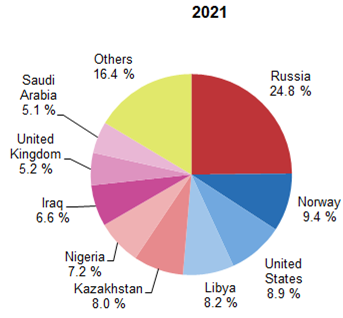
\includegraphics[width=0.60\textwidth]{images/eu oil import 21.png}
         \caption{EU imports of petroleum oil}
         \label{fig:eu oil import 21}
     \end{subfigure}
     \hfill
     \begin{subfigure}[b]{0.45\textwidth}
         \centering
         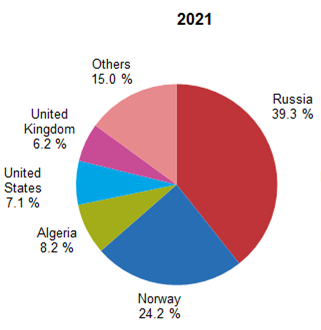
\includegraphics[width=0.58\textwidth]{images/eu nat gas import 21.png}
         \caption{EU imports of natural gas}
         \label{fig:eu nat gas import 21}
     \end{subfigure}
     \hfill
        \caption{EU imports of petroleum oil and natural gas by partner 2021 (\citeauthor{eurostat_2022})}
        \label{fig:eu 21 flows}
\end{figure}

\begin{figure}[h]
    \centering
    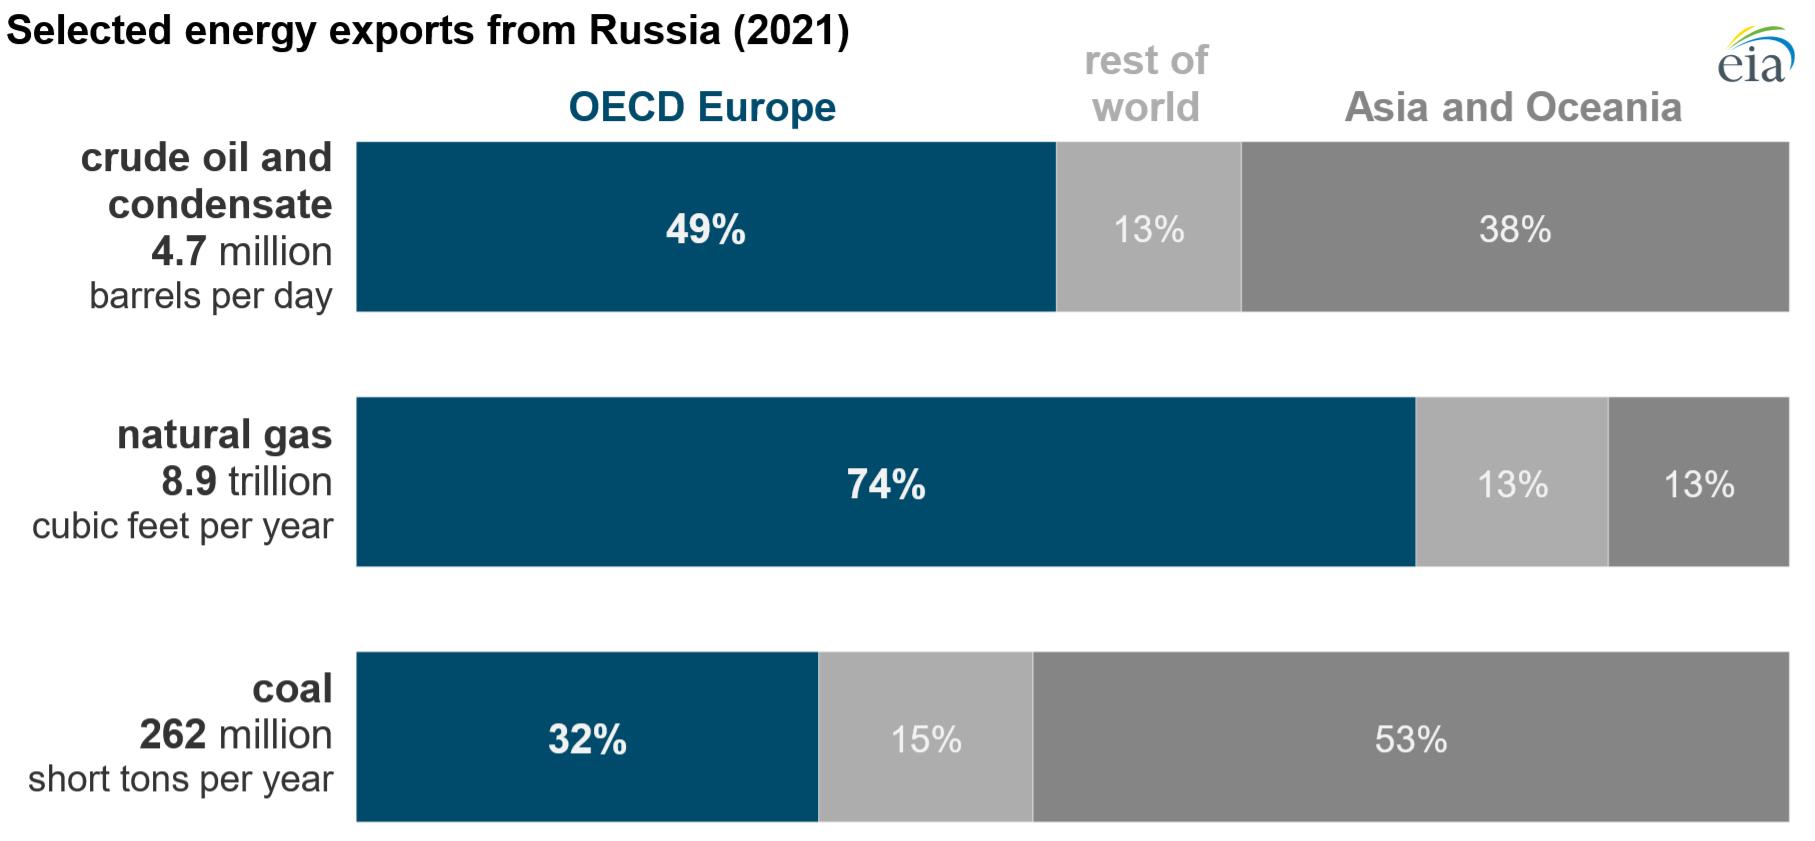
\includegraphics[width=0.5\textwidth]{images/rus exp 2021.png}
    \caption{Crude oil, natural gas and coal exports from Russia 2021 (\citeauthor{eia_2022})}
    \label{fig:rus exp 2021}
\end{figure}

With Russian crude oil averaging 10.8 million barrels produced and 3.7 million barrels consumed per day in 2021, approximately 7.1 million barrels per day are available for export, as illustrated in Figure \ref{fig:gas export avail} (\citeauthor{eia_2023}). Similarly, Figure \ref{fig:gas export avail} shows the amount of natural gas available for exports. Production in 2021 was 708 billion cubic meters, with 510 billion cubic meters consumed domestically, leaving 198 billion cubic meters for export (\citeauthor{eia_2023}). Figure \ref{fig:energy export avail} reveals an interesting relationship in Russian exports. Oil production has risen faster than consumption, leaving more oil available for export. By contrast, the volume of natural gas available for exports has remained relatively constant over the past 30 years. In addition, the figure shows that the majority of Russia's oil is exported, whereas the majority of Russia's natural gas is used for domestic consumption. 

\begin{figure}[h]
     \centering
     \begin{subfigure}[b]{0.45\textwidth}
         \centering
         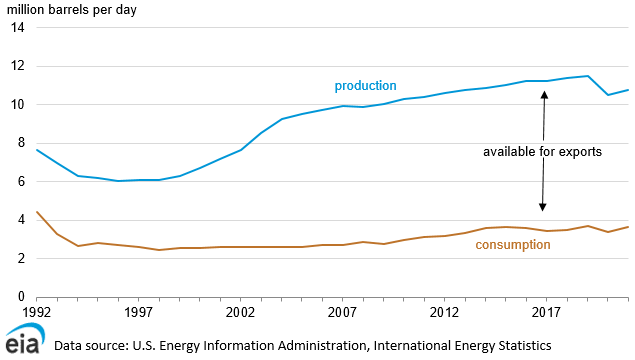
\includegraphics[width=0.8\textwidth]{images/oil export avail.png}
         \caption{Consumption and production of oil}
         \label{fig:oil export avail}
     \end{subfigure}
     \hfill
     \begin{subfigure}[b]{0.45\textwidth}
         \centering
         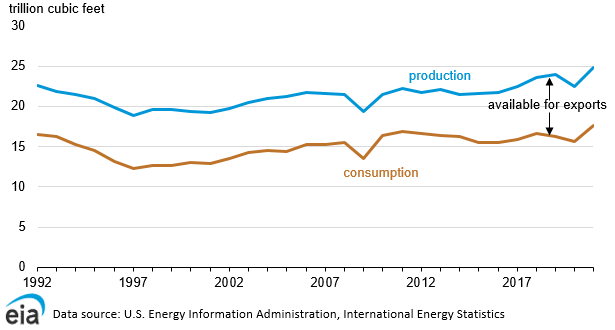
\includegraphics[width=0.8\textwidth]{images/gas export avail.png}
         \caption{Consumption and production of natural gas}
         \label{fig:gas export avail}
     \end{subfigure}
     \hfill
        \caption{Russian oil and natural gas domestic production and consumption (\citeauthor{eia_2023})}
        \label{fig:energy export avail}
\end{figure}

Russia's primary oil trade partner in 2021 was the EU, with 44\% of Russia's crude oil exports being transported to the EU by pipelines or by sea. However, China also imported a very large share of Russian crude oil, trailing close behind the EU with 30\% of Russia's exports. These distributions are summarised below in Figure \ref{fig:21 trade part}. 

\begin{figure}[h]
     \centering
     \begin{subfigure}[b]{0.45\textwidth}
         \centering
         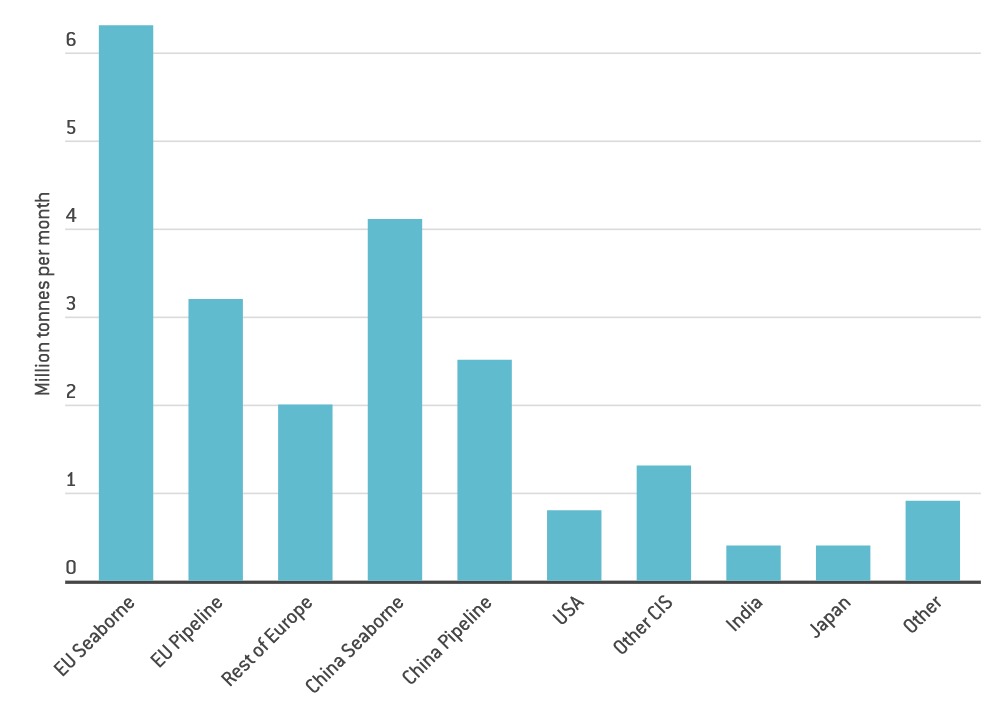
\includegraphics[width=0.53\textwidth]{images/21 trade part chart.png}
         \caption{Exports by volume}
         \label{fig:21 trade part chart}
     \end{subfigure}
     \hfill
     \begin{subfigure}[b]{0.45\textwidth}
         \centering
         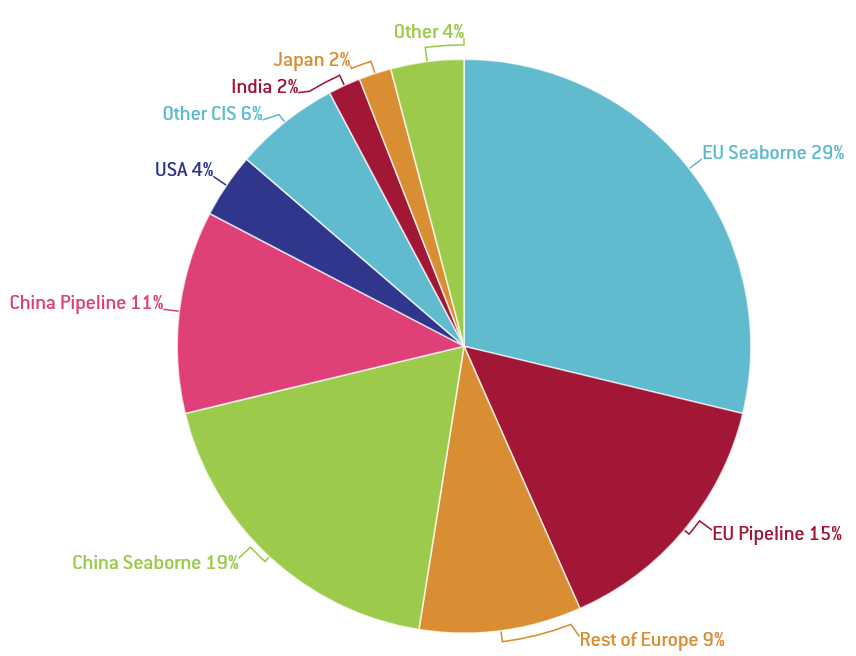
\includegraphics[width=0.53\textwidth]{images/21 trade part pie.png}
         \caption{Exports by share}
         \label{fig:21 trade part pie}
     \end{subfigure}
     \hfill
        \caption{Russian Monthly Average Crude Oil Exports 2021 (\citeauthor{heussaff_guetta-jeanrenaud_mcwilliams_zachmann_2023})}
        \label{fig:21 trade part}
\end{figure}

Within the EU, Germany, Netherlands and Poland imported the most crude oil and natural gas in 2021, importing 687, 414 and 372 thousand barrels per day, respectively (\citeauthor{reuters_2022}). It is also key to note which countries were most reliant on Russian crude oil, that is to say, for which countries does Russia account for the highest percentage of their imports? The most heavily exposed countries were Lithuania, with 83\% of crude oil imports from Russia, Finland with 80\%, and Slovakia with 74\% (\cite{reuters_2022}). The other side of the story is natural gas. As discussed previously, 74\% of Russia's natural gas in 2021 went to the EU. Notable importers of natural gas from Russia in 2021 were Belarus, taking 7.9\% of Russia's exports, and China taking 6.3\% (RM \citeauthor{rm_staff_2022}). This is due to the limitations of natural gas, where it can only be exported through pipelines unless it is converted to liquefied natural gas (LNG). In this regard, Russian natural gas exports are bound to some degree to its existing pipeline infrastructure, naturally favoring geographical neighbours.

Subsequently, we can see the interdependent nature of the European Union and Russia in the crude oil and natural gas industries, where the EU as a whole, and even more so, specific nations within the common market, relied on Russian imports for energy. However, the other side of the coin is that Russia also relied on exporting to the EU for revenue, particularly in natural gas.  
  
\section{European Union Sanctions}

Since the start of the Russo-Ukrainian war in February 2014, the European Union and various other countries have implemented sanctions against Russia. While EU sanctions in 2014 largely focused on the financial sector along with limitations on military equipment trade and investments in oil production (\citeauthor{the_council_of_the_european_union_2014}), the EU expanded these sanctions following the Ukrainian invasion of February 2022 rolling out increasingly restrictive sanctions against Russia. In relation to the energy sector, bans on energy production technology were tightened, followed by a ban on coal and solid fossil fuels in April, then crude oil and petroleum products in June (\citeauthor{dete_2022}). For the crude oil ban, the EU stated that a transitional period of 8-10 months would be provided only to specific nations with geographical limitations and strong dependency on Russian oil. The goal of these sanctions was to target one of Russia's major industries by forcing a change in trade partners: crude oil and natural gas. The two most relevant sanctions for this investigation from the Official Journal of the European Union are:

\begin{quote}
    "It shall be prohibited to sell, supply, transfer, or export, directly or indirectly, goods and technology suited for use in oil refining and liquefaction of natural gas, whether or not originating in the Union, to any natural or legal person, entity or body in Russia or for use in Russia." \\
    ---\textit{COUNCIL REGULATION (EU) 2022/576 \\ 8 April 2022}
\end{quote}

\begin{quote}
    "Imposing prohibitions on the purchase, import or transfer into Member States, directly or indirectly, of crude oil and certain petroleum products, which originate in Russia or are exported from Russia, and on the insurance and reinsurance of maritime transport of such goods to third countries. Appropriate transitional periods are provided for." \\
    ---\textit{COUNCIL REGULATION (EU) 2022/879 \\ 3 June 2022}
\end{quote}

The EU sanctions act upon previous 2014 sanctions and introduce the new crude oil ban, forcing Russia to change their trade partners, as well as prohibiting Liquefied Natural Gas (LNG) technology. Interestingly, the EU did not explicitly sanction natural gas, but by sanctioning the technology, they force Russia into a situation where it becomes difficult to export natural gas outside of existing pipelines, which mostly go to Europe. 

\section{Analysing the Impact}

\subsection{Changes in European Union Imports}

In accordance with the EU Sanctions, there has been a marked decrease in imports of Russian crude oil and natural gas by the European Union. Sanctions constitute an administrative barrier to trade. In the case of the EU, the sanctions have significantly reduced Russian crude oil and natural gas imports in the short-term. In the long-term, the EU aims to completely eliminate Russian crude oil and natural gas from its market. 

As shown in Figure \ref{fig:eu oil import}, within less than a year after the Ukraine invasion in 2022, crude petroleum oil imports by the EU were reduced from 25.9\% of EU imports in the second quarter of 2022 to 14.4\% in the third quarter. To enable this reduction, EU imports from Saudi Arabia rose from 4.8\% in the second quarter of 2022 to 9.1\% in the third quarter. Iraq, Norway and the United States all increased slightly. There was also a notable increase in crude oil imports from other countries, which rose from 15.1\% in the second quarter of 2022 to 24\% in the third quarter. These are countries for which individual nations' shares are not significant enough to be listed. 

\begin{figure}[h]
    \centering
    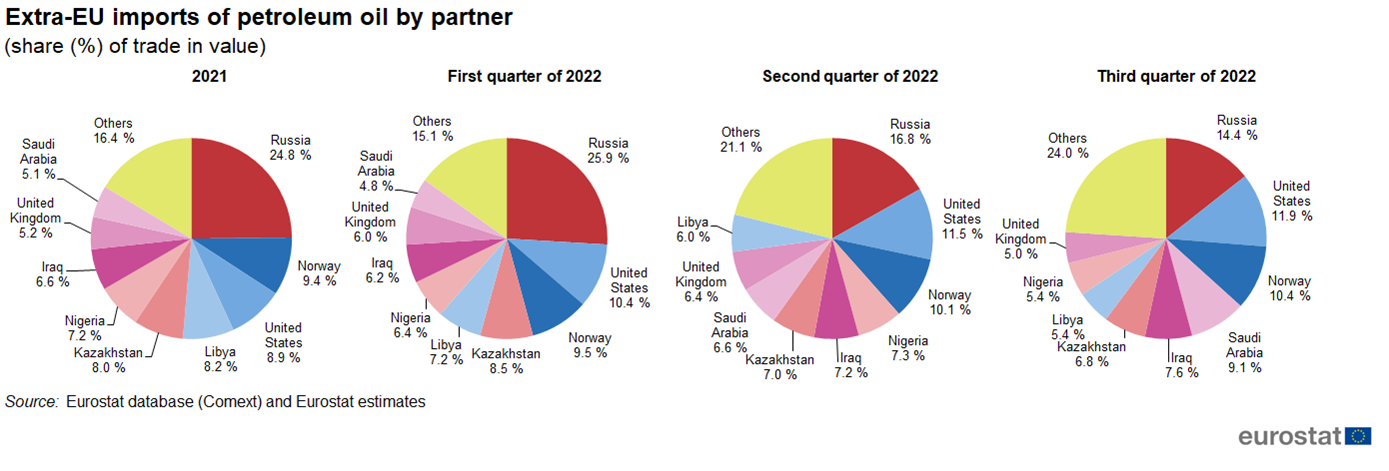
\includegraphics[width=\textwidth]{images/eu oil import.png}
    \caption{EU imports of petroleum oil by partner 2019-2021 (\citeauthor{eurostat_2022})}
    \label{fig:eu oil import}
\end{figure}

However, as a whole they have contributed significantly to the reallocation of petroleum oil imports. In parallel to crude oil, it can be seen in Figure \ref{fig:eu nat gas import} that natural gas imports from Russia also saw a significant decrease, dropping from 39.3\% of EU natural gas imports in 2021 to 15\% in the third quarter of 2022, more than halving. To replace Russian natural gas, there was a large increase in gas imported from Norway and the United Kingdom. As part of the reallocation of market share, Qatar became significant to the EU markets, providing 7.2\% of EU imports.

\begin{figure}[h]
    \centering
    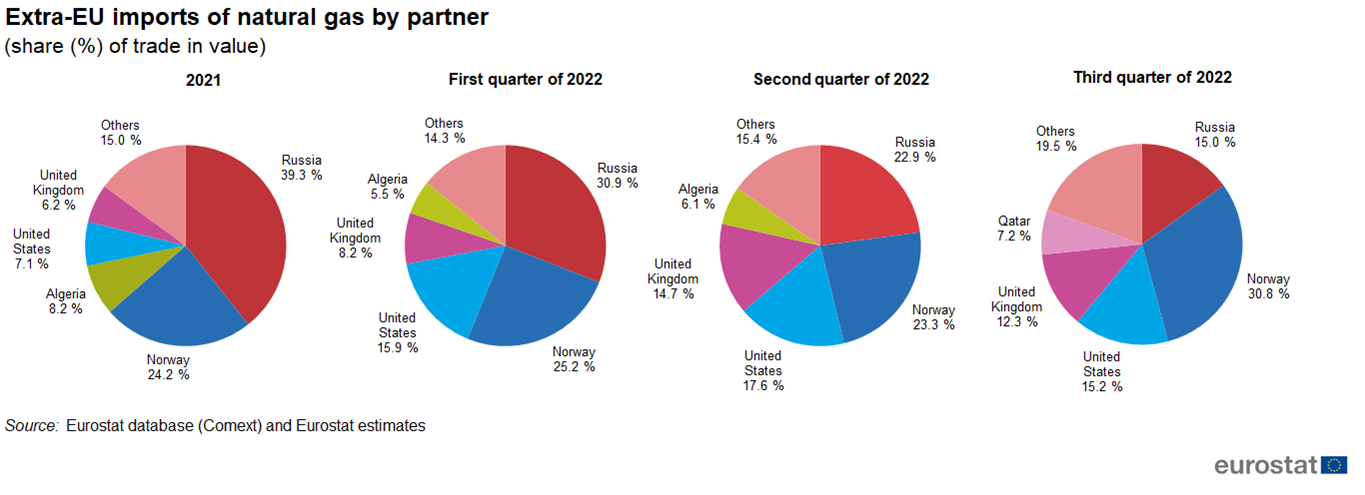
\includegraphics[width=\textwidth]{images/eu nat gas import.png}
    \caption{EU imports of natural gas by partner 2019-2021 (\citeauthor{eurostat_2022})}
    \label{fig:eu nat gas import}
\end{figure}


While these sanctions from the EU have been effective in the short term, with an immediate and significant decrease in imports of Russian crude oil and natural gas, this not a guaranteed outcome in the long term. The process is highly complex due to the necessity of energy in modern economies. As a union of 27 member states, each country faces unique challenges and this  can make the reduction of dependency on Russian energy products more difficult. Looking at the EU as a whole does not provide the full picture, and a more detailed analysis at the country level is needed.

According to Al Jazeera, nations like Denmark, Spain, Portugal, Sweden, Ireland and Austria were able to completely eliminate Russian oil from their import mix. Nations like Lithuania and Finland, which were heavily reliant on Russian oil (with over 80\% of imported oil being of Russian origin before the sanctions) successfully managed to reduce their importations to less than 10\%. However, not all nations have been so successful. In Slovakia, which was previously the third most dependent nation on Russian oil, the share of Russian crude oil imports grew to over 80\%. Likewise, in Hungary, Czechia and Italy, the share of Russian crude oil imports in their respective markets rose.

\begin{figure}[h]
    \centering
    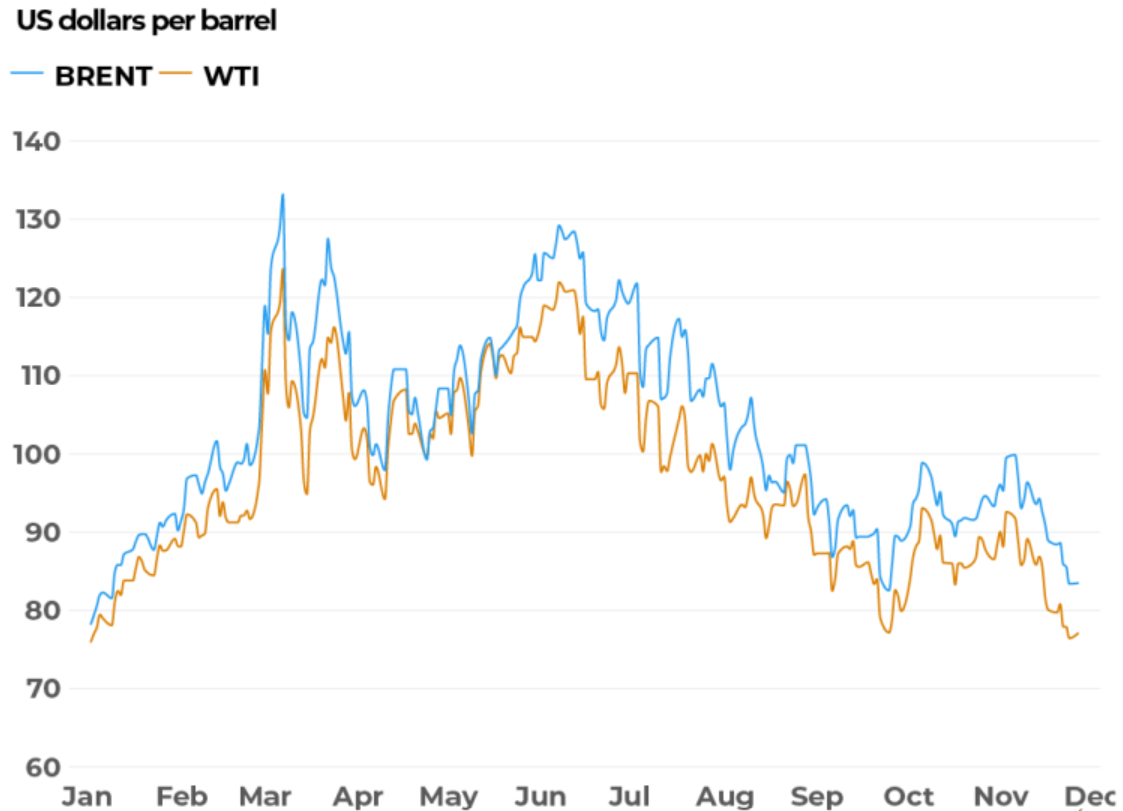
\includegraphics[width=0.45\textwidth]{images/oil prices.png}
    \caption{Oil prices in 2022 (Al \citeauthor{al_jazeera_2022})}
    \label{fig:oil prices}
\end{figure}

As nations are being forced to make sudden shifts in trade partners and find alternative sources for energy, notably moving towards LNG imports, the costs for energy rise, as seen in the rise of oil prices in Figure \ref{fig:oil prices}. The sharp peak in March directly followed the Ukrainian invasion. The steady rise in prices until the summer of 2022 can be explained by increasing energy scarcity due to supply constraints and trade diversion in the context of a strong world economy, compounded by Russia ceasing to be considered a reliable supplier. However, as EU nations, and the world as a whole, adapted to the new supply chains, prices began to settle down. 

Demand for crude oil and natural gas is relatively inelastic in the short run as changing the energy supply chain is a costly exercise in both the short and the long term, since these resources are difficult to replace for both consumption and industry use. This is illustrated in Figure \ref{fig:inelast} where because the EU demand for energy resources is so inelastic, large changes in price (from $P_1$ to $P_2$) as exemplified by the oil price spikes, have little effect on the equilibrium quantity which only decreases from $Q_1$ to $Q_2$. However, it's important to recognise how time can increase elasticity, where consumer and industry uses can be expected to adjust with greater force towards a new equilibrium. This is demonstrated in how the EU's reevaluation of trade partners over the 6-months following the invasion, resulted in a decrease in oil prices because there were more substitutes available for Russian energy, thus increasing the market size.  

\begin{figure}[h]
    \centering
    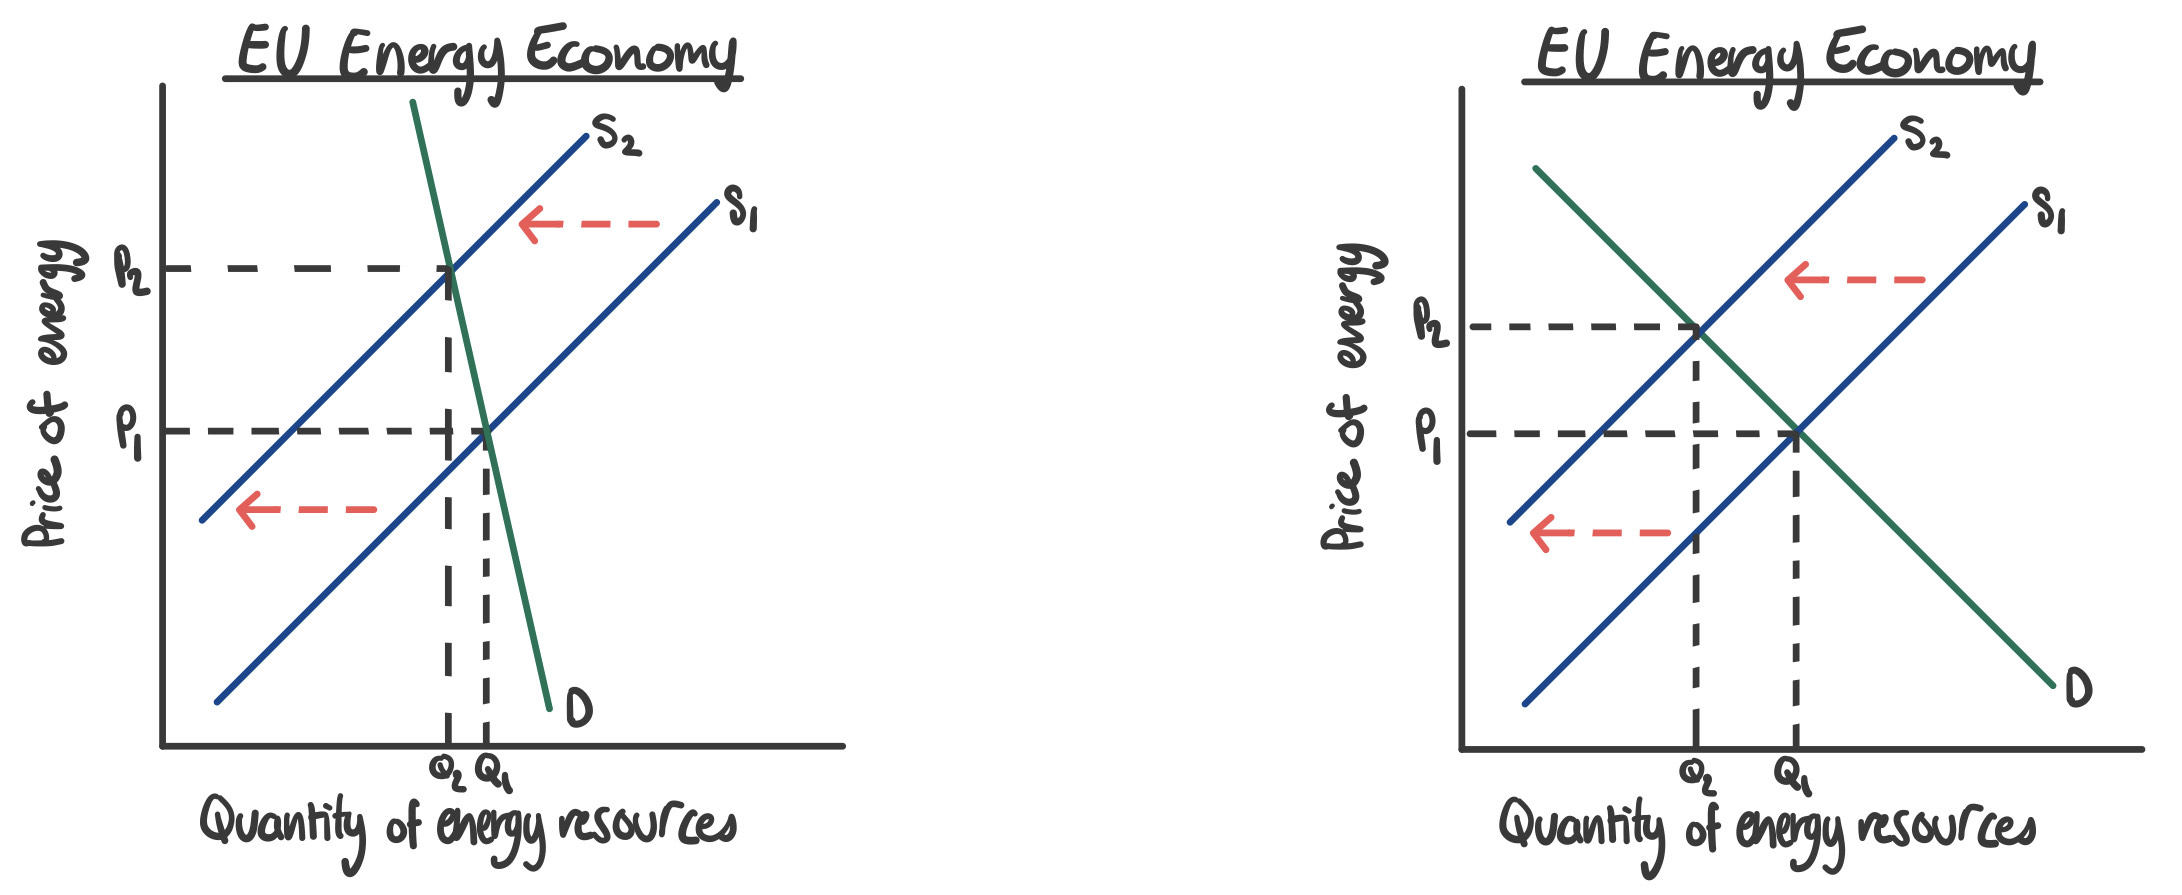
\includegraphics[width=0.9\textwidth]{images/a inelast.jpg}
    \caption{Market for Energy in the European Union}
    \label{fig:inelast}
\end{figure}

This demonstrates an important characteristic of EU nations. EU nations were highly dependent on Russian oil and natural gas prior to the Ukrainian invasion and the onset of the sanctions. However, because these nations had the economic resources to maintain energy security, albeit at higher cost, the sanctions could be implemented effectively. There is no question that this implied a heavy cost to these economies. Examples included forced energy usage reduction paired with high energy prices. Such higher costs were passed onto consumers in almost every product as energy is an essential factor of production. However, it is for this very reason that the sanctions are likely to be even more effective in the long-term: More permanent alternatives to Russian energy are likely to become available to the EU, including not only new trade partners, but also a rise in sustainable energy development. 

\subsection{Russian Crude Oil and Natural Gas Production}

Russia's dependency on the European market for crude oil and natural gas exports meant that the significant reduction in sales to the EU had significant impacts on Russia's oil production, where volume produced took a heavy toll. 

\begin{figure}[h]
    \centering
    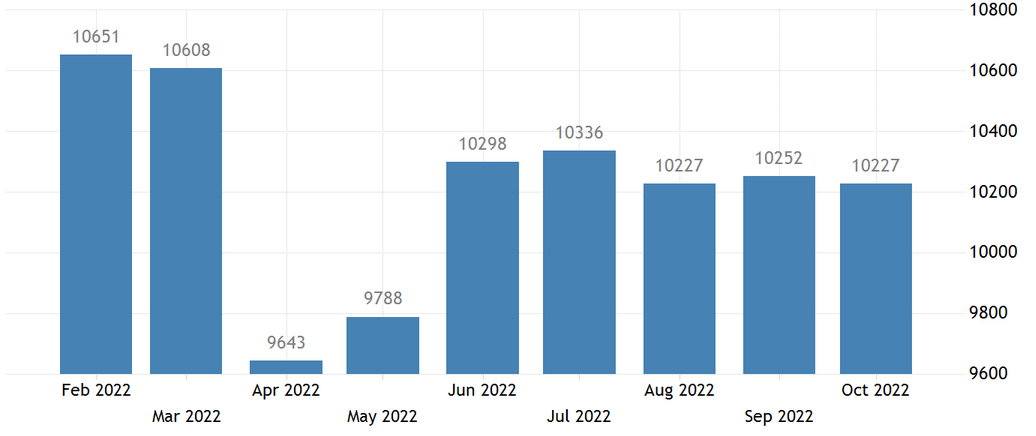
\includegraphics[width=0.6\textwidth]{images/oil prod.png}
    \caption{Russian oil production in 2022, kbpd (Trading \citeauthor{trading_economics})}
    \label{fig:oil prod}
\end{figure}

Figure \ref{fig:oil prod} shows that Russia saw a large decrease in oil production as the effects of the invasion began to take a toll on oil production, which fell from 10.6 million barrels per day to 9.6 million barrels per day in April. However, it's important to note the axis provided on this graph which seems to exaggerate the effect of this oil production fall. It is seen that production recovered in the following months, but did not return to the levels prior to the invasion, settling at around 10.2 million barrels per day. This can be seen as a direct impact of the sanctions implemented by the EU and other nations. Russia has been forced to reduce production because of curtailed demand from its former key markets, and while the process of trade diversion continues, it is still incomplete.  

For Russia's natural gas sector, the effects are stronger. Although the EU did not sanction natural gas as severely as oil, EU imports of natural gas dropped dramatically. Natural gas is difficult to divert as it can only be transported through pipelines or sold as LNG, a more costly and complex process. Russia has extensive pipelines within Europe - infrastructure that has taken decades to build and develop, as seen in Figure \ref{fig:pipelines}. Although Russia has extensive infrastructure to convert natural gas into LNG, the EU also sanctioned all LNG technology, making the expansion of the LNG industry in Russia much more difficult, if not altogether infeasible.

\begin{figure}[h]
    \centering
    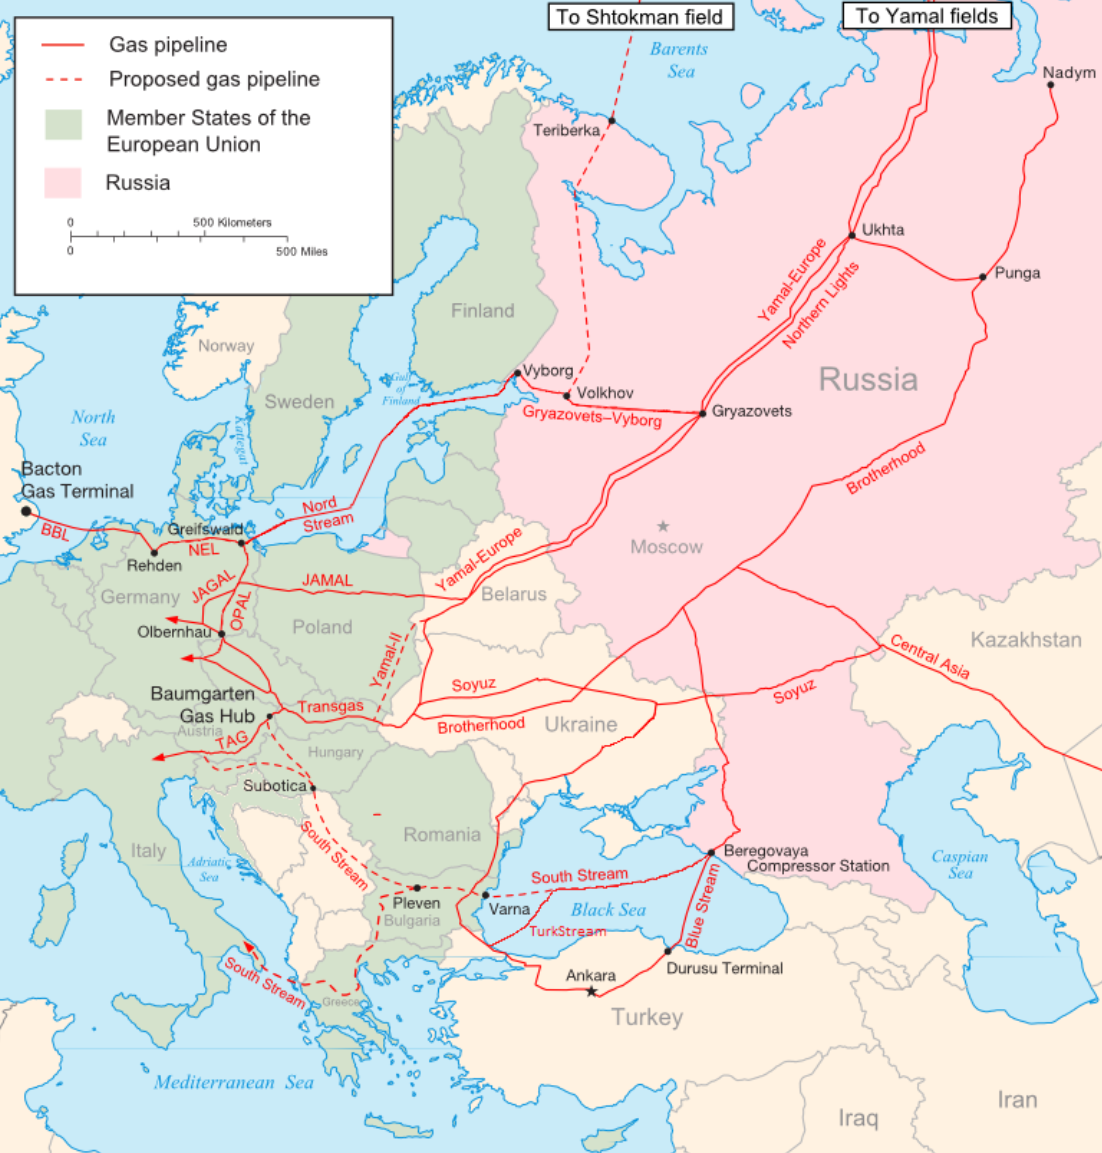
\includegraphics[width=0.4\textwidth]{images/pipelines.png}
    \caption{Russian gas pipelines in Europe (\citeauthor{conca_2014})}
    \label{fig:pipelines}
\end{figure}

\vspace{-5mm}

Consequently, natural gas production fell for three consecutive months after the invasion, reaching an 18\% fall by June of 2022, and remaining at 70\% of March 2022 production levels (\citeauthor{ief_2022}). This is not surprising given that the EU accounted for 74\% of Russia's natural gas exports, and since EU imports fell by more than half, Russia has had to reduce production. As a large industry for Russia, a reduction in production of natural gas is a clear indicator of declining productivity as Russia's export flows change with their trade partners, and subsequently a decline in exports forces a decline in production. 

\subsection{Revenue in Respective Russian Industries}

Revenue is the product of volume sold and the price at which it is sold. Although crude oil production was at an extreme low for Russia in March 2022 as seen in Figure \ref{fig:oil prod}, prices also spiked to a high point as seen in Figure \ref{fig:oil prices}. 

\begin{figure}[h]
    \centering
    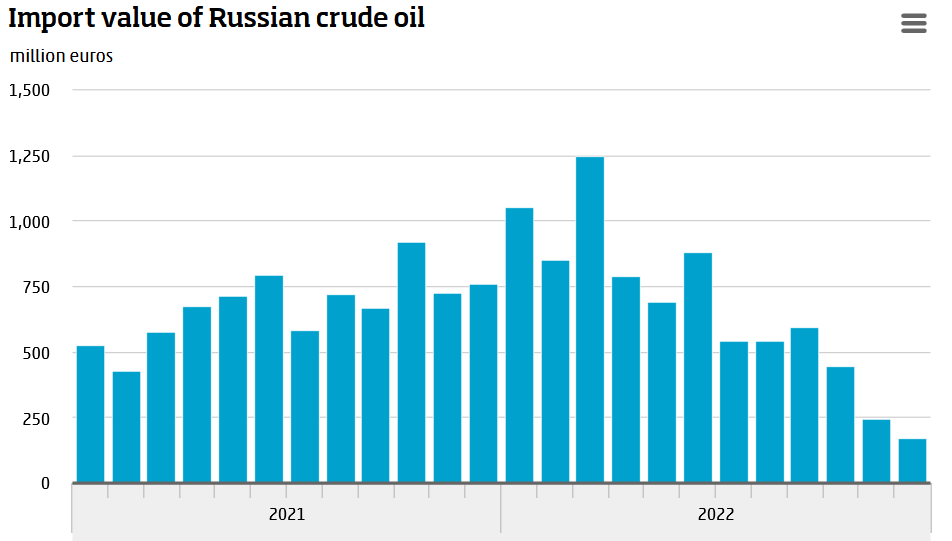
\includegraphics[width=0.55\textwidth]{images/import value.png}
    \caption{Import value of Russian crude oil in million euros (\citeauthor{})}
    \label{fig:import value}
\end{figure}

Logically, this follows the law of supply by which if supply decreases, then prices increase: The supply of oil decreased due to of demand decreasing, where the size of the market Russia could sell to suddenly became smaller as the EU sanctioned Russian oil. This is illustrated in my graph below, Figure \ref{fig:ds}, showing how the initial contraction in demand, from $D_1$ to $D_2$ caused movement down the Supply curve, which then lead to a contraction in supply, resulting in a price increase. 

\begin{figure}[h]
    \centering
    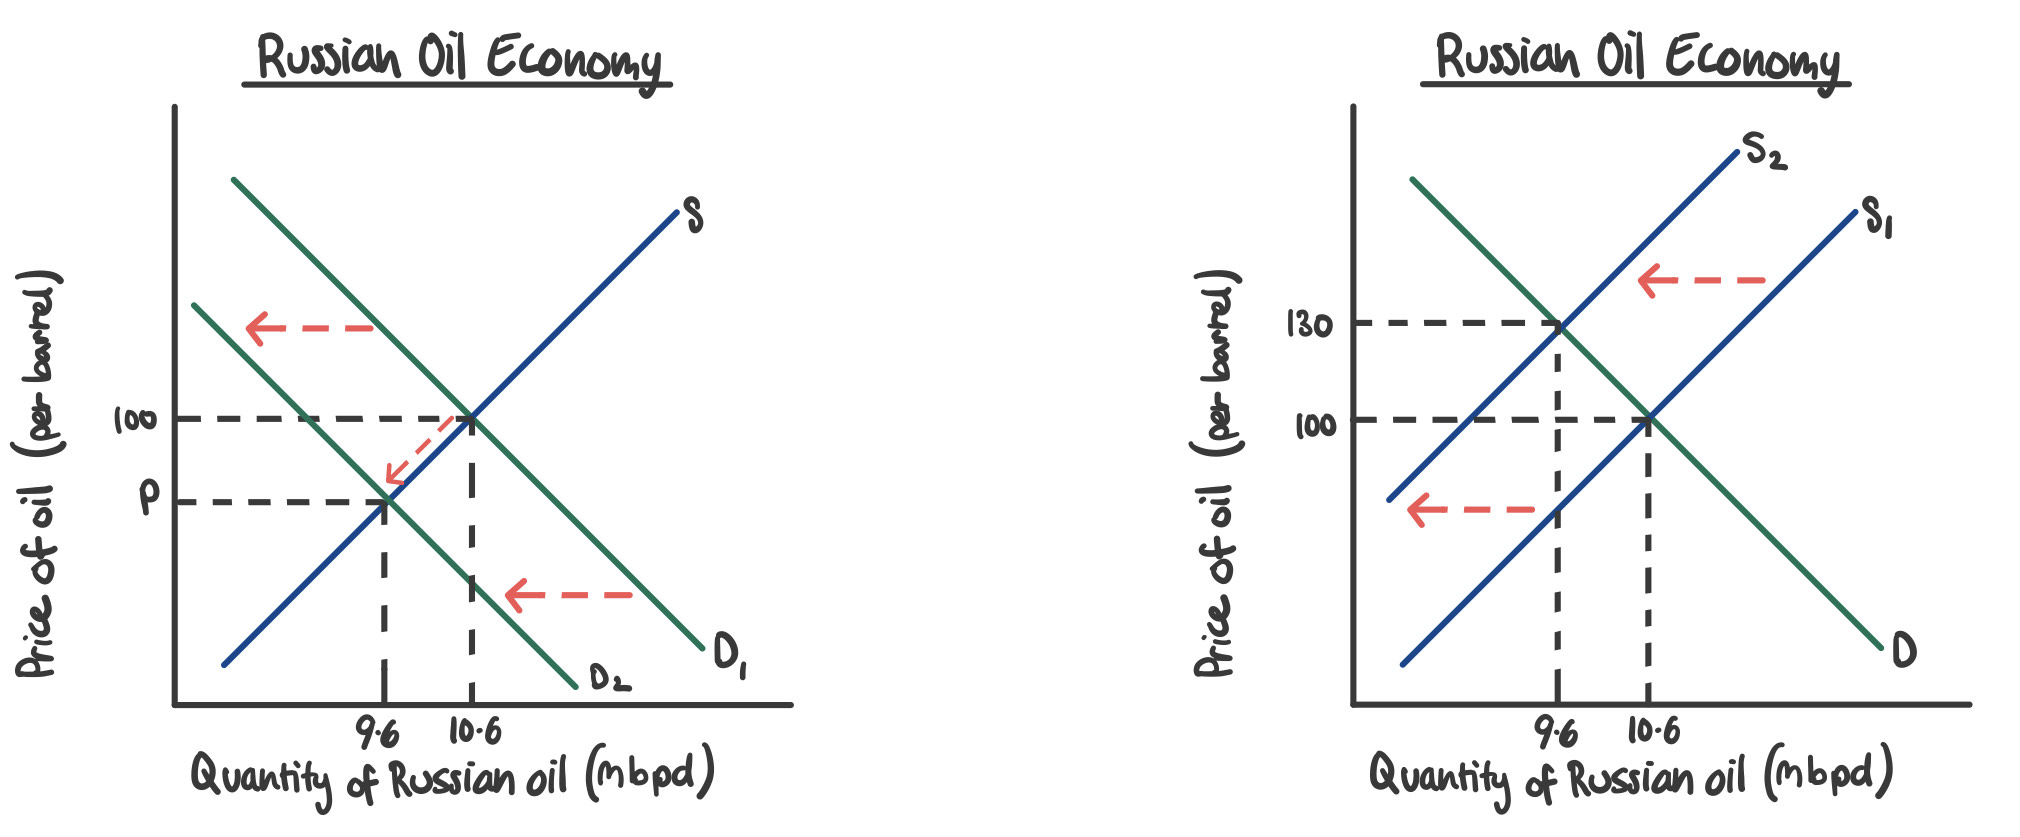
\includegraphics[width=0.7\textwidth]{images/a graph ds.jpg}
    \caption{Russian oil economy showing oil volume supplied and price}
    \label{fig:ds}
\end{figure}

Because of this increase in price, the value, and thus revenue generated from exporting Russian crude oil suddenly increased as seen by the peak at 1,750 million euros in March 2022 on Figure \ref{fig:import value}. However, this period of Russia profiting from oil exports was short lived as prices settled back down but crude oil production settled below the original production level as seen in Figure \ref{fig:oil prod}. This demonstrates the key difference between the short-term and long-term effects of the EU sanctions: while the EU sanctions triggered a price hike, and subsequently raised Russian revenues in the short-term, in the long-term, they damaged Russian production, not allowing revenues to recuperate after prices settled. 

\subsection{Change in Trade Partners for Russia}

The EU's decreased crude oil and natural gas imports from Russia led to a drop in Russian production. To complete the picture, it is important to understand to which new markets Russia is selling their crude oil and natural gas. Russia has been increasing crude oil exports to China, which previously took 30\% of their exports. In addition to China, India has increased its Russian oil imports. Previously having only purchased 2\% of Russia's exports, India is now importing 20\% of Russia's crude oil exports (\citeauthor{iea}). Turkey has also doubled their Russian crude oil imports as seen in the chart below, Figure \ref{fig:trade change}.

\begin{figure}[h]
    \centering
    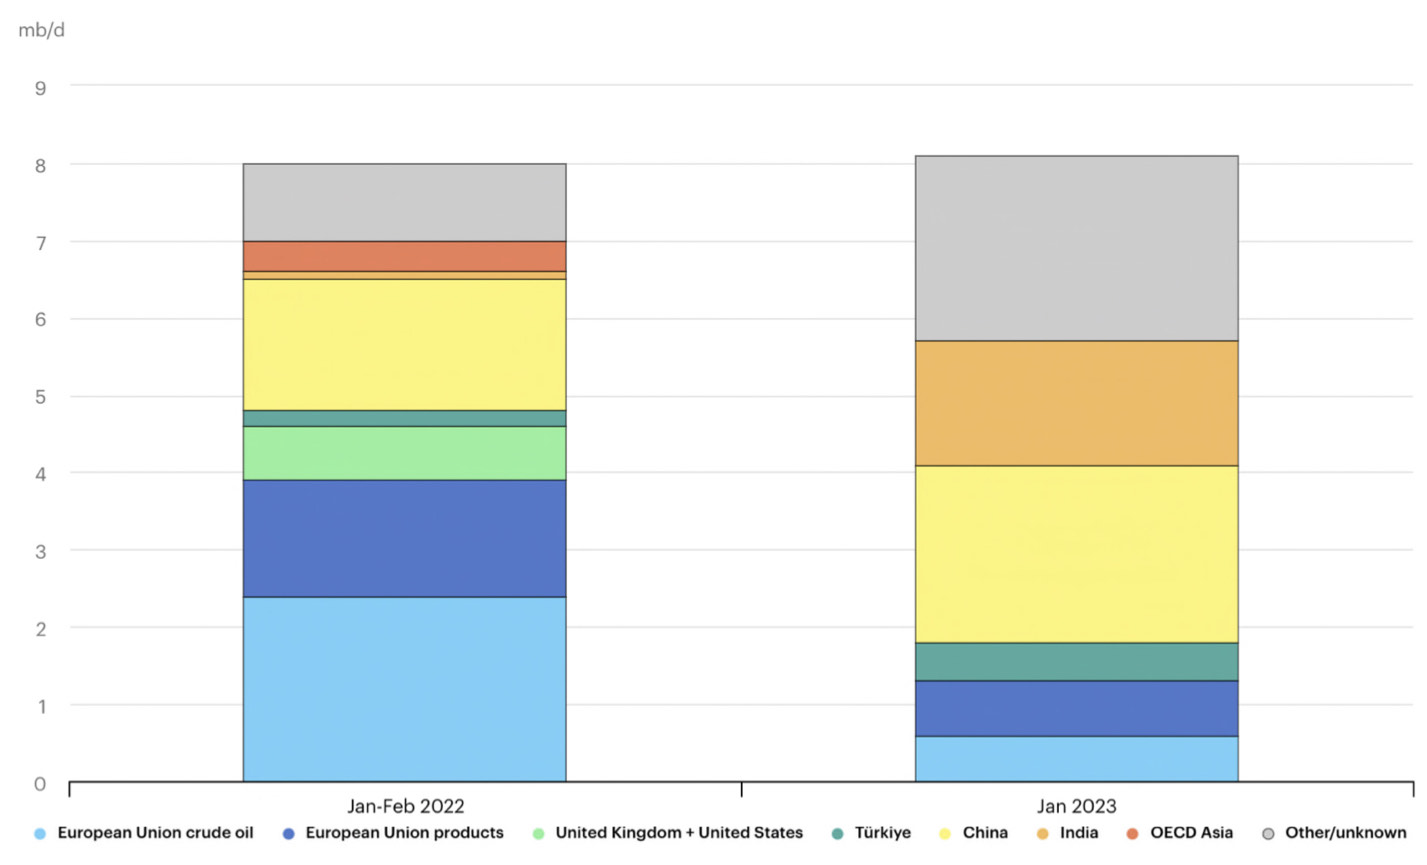
\includegraphics[width=0.6\textwidth]{images/trade change.jpg}
    \caption{Russia's crude oil exports by region (\citeauthor{iea})}
    \label{fig:trade change}
\end{figure}

However, since natural gas cannot be easily exported without infrastructure or converting it into LNG, prospects for Russia's gas exports are not positive, with some forecasts predicting massive reductions in natural gas by up to -180 billion cubic meters per year by 2025 (\citeauthor{iea_2022_journal}). 

Overall, Russia was able to successfully and swiftly change crude oil exports by changing trade partners and maintain a relatively steady production and exportation. However, they have not yet successfully redirected natural gas exports, which previously went to the EU, because they lack the technology to expand the LNG industry which would allow for the mobilisation of natural gas. 

\section{Conclusion}

One year after the invasion, the long-term effects of the sanctions are starting to take place as Russia's crude oil and natural gas industry are heading into a decline despite efforts to maintain them afloat. 

Russia's early response to the sanctions by expanding crude oil sales to India, China and Turkey brought significant benefits, particularly as seen at the start of the sanctioning period, in early March 2022. By capitalising on high prices, Russia was able to generate more revenue than before, despite lower production, where it seemed as if the sanctions were only negatively impacting the European Union. However, this effect was short lived as oil prices settled and the aftermath of lower production caused Russia's revenues to drop again: Russia's oil and gas sector is beginning to show some signs of decline. 

From the European Union's perspective, despite economic barriers faced by some nations that were unable to reduce Russian energy imports, the EU as a whole managed to decrease crude oil and natural gas imports by about half in only two quarters - a relatively fast response. Yet the EU had no choice but to switch to more expensive energy sources as supply chains rapidly readjusted.  

\pagebreak

\printbibliography
 
\end{document}